\documentclass[twocolumn]{aastex631}

% Packages
\usepackage{microtype}  % ALWAYS!
\usepackage{amsmath}
\usepackage{amsfonts}
\usepackage{amssymb}
\usepackage{multirow}

\newcommand{\mlg}{M$_{\rm LG}$}
\definecolor{pink}{RGB}{232,132,161}
\newcommand{\kc}[1]{\textcolor{pink}{\textbf{#1}} }
\newcommand{\mud}{\mu_\delta}
\newcommand{\mua}{\mu_\alpha^*}

% Style tweaks
% \renewcommand{\twocolumngrid}{\onecolumngrid}
% \setlength{\parindent}{1.1\baselineskip}
% \sloppy\sloppypar\raggedbottom\frenchspacing


%%%%%%%%%%%%%%%%%%%%%%%%%%%%%%%%%%%%%%%%%%%%%%%%%%%%%%%%%%%%%%%%%%%%%%%%%%%%%%%%
\shorttitle{Updated Local Group Mass from Timing Argument}
\shortauthors{Chamberlain, Price-Whelan et al.}

%%%%%%%%%%%%%%%%%%%%%%%%%%%%%%%%%%%%%%%%%%%%%%%%%%%%%%%%%%%%%%%%%%%%%%%%%%%%%%%%
\graphicspath{{./}{figures/}}
% Missions
\newcommand{\project}[1]{\textsl{#1}}

% Packages / projects / programming
\newcommand{\package}[1]{\textsl{#1}}
\newcommand{\acronym}[1]{{\small{#1}}}
\newcommand{\github}{\package{GitHub}}
\newcommand{\python}{\package{Python}}
\newcommand{\astropy}{\package{Astropy}}

% Stats / probability
\newcommand{\given}{\,|\,}
\newcommand{\norm}{\mathcal{N}}
\newcommand{\pdf}{\textsl{pdf}}

% Maths
\newcommand{\dd}{\mathrm{d}}
\newcommand{\transpose}[1]{{#1}^{\mathsf{T}}}
\newcommand{\inverse}[1]{{#1}^{-1}}
\newcommand{\argmin}{\operatornamewithlimits{argmin}}
\newcommand{\mean}[1]{\left< #1 \right>}

% Non-scalar variables
\renewcommand{\vec}[1]{\ensuremath{\bs{#1}}}
\newcommand{\mat}[1]{\ensuremath{\mathbf{#1}}}

% Unit shortcuts
\newcommand{\Msun}{\ensuremath{\mathrm{M}_\odot}}
\newcommand{\Mjup}{\ensuremath{\mathrm{M}_{\mathrm{J}}}}
\newcommand{\kms}{\ensuremath{\mathrm{km}~\mathrm{s}^{-1}}}
\newcommand{\pc}{\ensuremath{\mathrm{pc}}}
\newcommand{\kpc}{\ensuremath{\mathrm{kpc}}}
\newcommand{\Mpc}{\ensuremath{\mathrm{Mpc}}}
\newcommand{\kmskpc}{\ensuremath{\mathrm{km}~\mathrm{s}^{-1}~\mathrm{kpc}^{-1}}}
\newcommand{\dayd}{\ensuremath{\mathrm{d}}}
\newcommand{\yr}{\ensuremath{\mathrm{yr}}}
\newcommand{\Kel}{\ensuremath{\mathrm{K}}}

% Misc.
\newcommand{\bs}[1]{\boldsymbol{#1}}

% Astronomy
\newcommand{\DM}{{\rm DM}}
\newcommand{\feh}{\ensuremath{{[{\rm Fe}/{\rm H}]}}}
\newcommand{\df}{\acronym{DF}}

% TO DO
\newcommand{\todo}[1]{{\color{red} TODO: #1}}
\newcommand{\apw]}[1]{{\color{green} APW says: #1}}

% Projects
\newcommand{\gaia}{\textsl{Gaia}}
\newcommand{\gaiadr}{\textsl{Gaia}~\acronym{EDR3}}


% Affiliations
\newcommand{\affuofa}{University of Arizona, 933 N. Cherry Ave,
    Tucson, AZ 85721, USA}
\newcommand{\affcca}{Center for Computational Astrophysics, Flatiron Institute,
    Simons Foundation, 162 Fifth Avenue, New York, NY 10010, USA}

%% This is the end of the preamble.  Indicate the beginning of the
%% manuscript itself with \begin{document}.

\begin{document} 

\title{
    A timing argument mass for the Local Group accounting for the
    Milky Way--LMC reflex motion
}

\author[0000-0001-8765-8670]{Katie~Chamberlain}
\affiliation{\affuofa}

\author[0000-0003-0872-7098]{Adrian~M.~Price-Whelan}
\affiliation{\affcca}

\author{Others!}


\begin{abstract}
    % \textbf{Context} 
    The Local Group mass sets the distribution and kinematics of its constituent galaxies and is necessary to place it in a cosmological context. Though challenging to measure, one method that has been used to estimate the Local Group mass is the Timing Argument, which constructs a Keplerian orbital model that is matched to the observed kinematics of M31 with respect to the Milky Way. 
    However, recent observations of stellar tracers in the outer MW halo have revealed an excess velocity dipole in the radial velocities that can be interpretted as a bulk motion of the Milky Way disk with respect to its outer halo. 
    This motion of the disk has previously been unaccounted for in Timing Argument models. 
    % \textbf{Aims} 
    We aim to infer a Local Group mass that accounts for the reflex motion of the Milky Way disk.    
    % \textbf{Methods} 
    We use Bayesian techniques to fit collected datasets of 6D phase-space information of M31 and determine the dependence of the inferred Local Group mass on the magnitude of the reflex motion.
    % \textbf{Results} 
    We provide an updated Local Group mass of $4.69\pm0.71 \times 10^{12}$M$_\odot$ assuming a disk travel velocity of $32\rm km/s$. 
    Additionally, we find that the inclusion of the reflex motion of the MW disk systematically lowers the inferred Local Group mass via the Timing Argument, and that the recovered mass depends strongly on the assumed travel velocity of the disk.
    Further measurements of the reflex motion of the disk will likely yield a larger observed travel velocity, and therefore a lower Local Group mass. In addition, improvements to proper motion measurements from future Gaia data releases may improve the constraint on the Local Group mass by a factor of $\sim2$.
    % \textbf{Conclusions}
    The Timing Argument remains one of the only ways to measure the Local Group mass independently of the masses of the individual component galaxies, but it is clear that the effect of the LMC must be accounted for when using these techniques. 

\end{abstract}

\section{Introduction}
\label{sec:intro}

\begin{itemize}
    \item importance of knowing mass of the local group
    \item ways to measure local group mass
    \item \begin{itemize}
            \item other tracers? 
            \item introduction of timing argument 
            \item what previous TA measurements of the local group mass have been
          \end{itemize}
    \item what's wrong with previous use of TA?
        \begin{itemize}
            \item the LMC is massive and pulling on the MW disk
            \item previous use of timing argument did not account for travel velocity of the disk
            \item we include the travel velocity of the disk
        \end{itemize}
    \item cosmological impact
        \begin{itemize}
            \item bias and calibration of the timing argument 
            \item what a lower/higher group mass means (we're gonna be more consistent w other group mass measurements, I think?)
        \end{itemize}
    
\end{itemize}

%%%%%%%%%%%%%%%%%%%%%%%%%%%%%%%%%%%%
\section{Methods}\label{sec:methods}
%%%%%%%%%%%%%%%%%%%%%%%%%%%%%%%%%%%%
In this section, we will discuss our coordinate system and the 

% THings that go into Keplerian assumption
% we can consider the dynamics of MW+M31 to be approximately simple because:
  % MW+M31 are far enough apart that the 
We first set up a coordinate system and model parameters 

Local Group dynamics are dominated by the local gravitational potential, and the Hubble flow can be neglected~\cite{}. Since M31 and MW 

On model parameters:


We can solve the equations of motion for a two body interaction analytically in the case of a Keplerian orbit:

\begin{equation}\label{eq:r}
  r = a(1-e\cos\eta)\\
\end{equation}

\begin{equation}\label{eq:t}
  t=\bigg(\frac{a^3}{GM}\bigg)^{1/2}(\eta-e\sin\eta)
\end{equation}

\begin{equation}\label{eq:vrad}
  v_{rad} = \bigg( \frac{a}{GM} \bigg)^{-1/2} \frac{e\sin\eta}{1-e\cos\eta}
\end{equation}

\begin{equation}\label{eq:vtan}
  v_{tan}= \bigg( \frac{a}{GM} \bigg)^{-1/2} \frac{\sqrt{1-e^2}}{1-e\cos\eta}.
\end{equation}
where, in our model, $r$ is the distance between M31 and the center of mass of the MW halo, $t$ is the time that has elapsed since the Big Bang (the current age of the Universe), and $v_{rad}$ ($v_{tan}$) is the radial (tangential) velocity of M31 toward the center of mass of the MW halo. 

Each of these observables can be translated to observables from the 

Important to note is that each of these is an observable of the motion of Andromeda

The dynamics of M31 and the MW are set in the case of a simple Keplerian orbit. In this case, their kinematics are completely set by 4 parameters: (\mlg, $a$, $e$, $\eta$) where \mlg is the mass of the Local Group, $a$, $e$, and $\eta$ are the semi-major axis, eccentricity, and eccentric anomaly of the orbit of M31 about the MW. 



In order to transform from the model parameters to these "observable quantities", 



% bit about how to include reflex velocity here.
We must account for the reflex motion of the MW disk with respect to its outer halo. We adopt the notation of~\cite{Penarrubia2016}, where $v_{A\to B}$ represents the velocity vector of \textit{A} as measured in the reference frame of \textit{B}. Thus, the observed velocity vector of M31 from the Galactic frame is given by:
\begin{equation}
  v_{\rm M31 \to \odot} = v_{\rm M31 \to \rm MW} + 
                          v_{\rm MW \to \rm \odot}
\end{equation}
However, the recent pericentric passage of the LMC has imparted a velocity boost on the disk and inner regions of the dark matter halo and disk of the Milky Way. Thus,
\begin{equation}
  v_{\odot \to \rm MW} = v_{\odot \to \rm MW_{D}} + v_{\rm MW_{D}\to \rm MW_{OH}} 
\end{equation}
where $v_{\rm MW_{D}\to \rm MW_{OH}}$ is the velocity vector of the center of the MW disk that is moving with travel velocity $v_{rm travel}$ from the reference frame of the barycenter of the outer, unperturbed dark matter halo of the MW.
Then, $v_{\odot \to \rm MW_{D}}$ is the velocity vector of the Sun about the MW disk center, given by 
\begin{equation}
  v_{\odot \to \rm MW_{D}}=({\rm U}_\odot, {\rm V}_\odot + V_0, {\rm W}_\odot)  
\end{equation}

% what are our model parameters?


We used \texttt{pymc3}~\citep{Salvatier2016} to sample from the 

Details about our pymc3 run like \# chains, steps, etc.




In order to translate between the 






%%%%%%%%%%%%%%%%%%%%%%%%%%%%%%%%%%%
\section{Datasets}
%%%%%%%%%%%%%%%%%%%%%%%%%%%%%%%%%%%
We use heliocentric radial velocities and proper motions. 

See~\ref{table:data} for values.
\begin{table}
  \centering
  \begin{tabular}{lc|c}
    \hline\hline
                    & Dataset 1                     & Dataset 2 \\\hline
  $D$               &  770 $\pm$ 40 \rm kpc\cite{}     &           \\
  $v_{\rm rad}$     &           &           \\
  $\mu_\alpha^*$    & 44.6$\pm$12.66\cite{} \\
  $\mu_\delta$      & -32.1$\pm$12.21 $\mu\rm as/yr$ & \\
  (U$_{\rm pec}$, V$_{\rm pec}$, W$_{\rm pec}$) & (11.1, 12.24, 7.25)& \\
  V$_0$             & 239.3$\pm$10.3 km/s & \\
  %              &           &           \\
  %              &           &           \\ 
  \hline\hline
  
  \end{tabular}
  \caption{Observational datasets used for comparison throughout analysis.}
\end{table}

% \footnote{note: Dataset 1 values of the proper motions are given as ($v_{w}, v_{N}$), then $(\mu_\alpha^*, \mu_\delta)$ were derived given $v_W=-\mua D$ and $v_N=\mud D$}

%%% Schematic %%%
\begin{figure*}[htb]
    \centering
    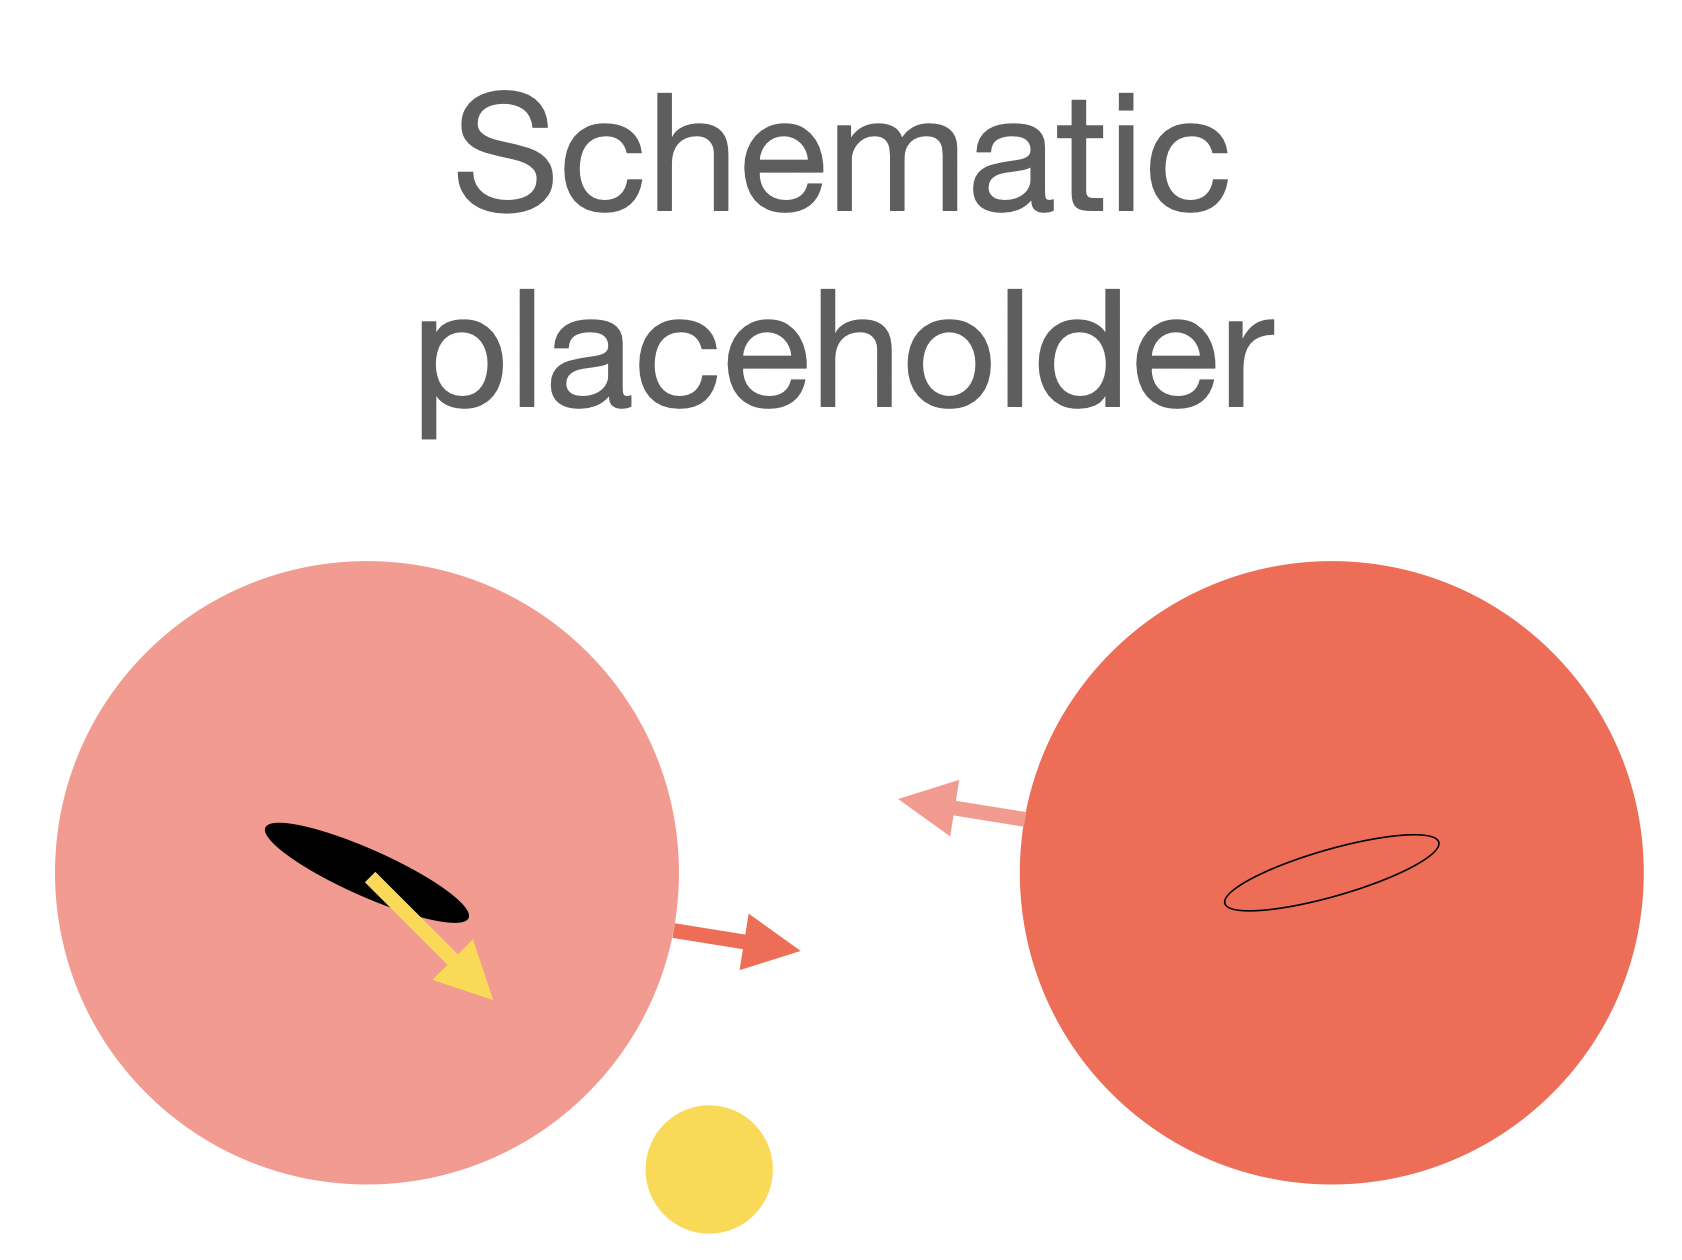
\includegraphics[width=0.8\columnwidth]{schematic_placeholder.png}
    \caption{\label{fig:schematic} Placeholder for whatever schematic we're going to end up creating
    }
  \end{figure*}

\kc{need tables with the data values and referencces for the observables used to constrain our model}

%%%%%%%%%%%%%%%%%%%%%%%%%%%%%%%%%%%
\section{Results: Local group mass estimates}
%%%%%%%%%%%%%%%%%%%%%%%%%%%%%%%%%%%
\label{sec:results}

\begin{figure*}[htb]
  \centering
  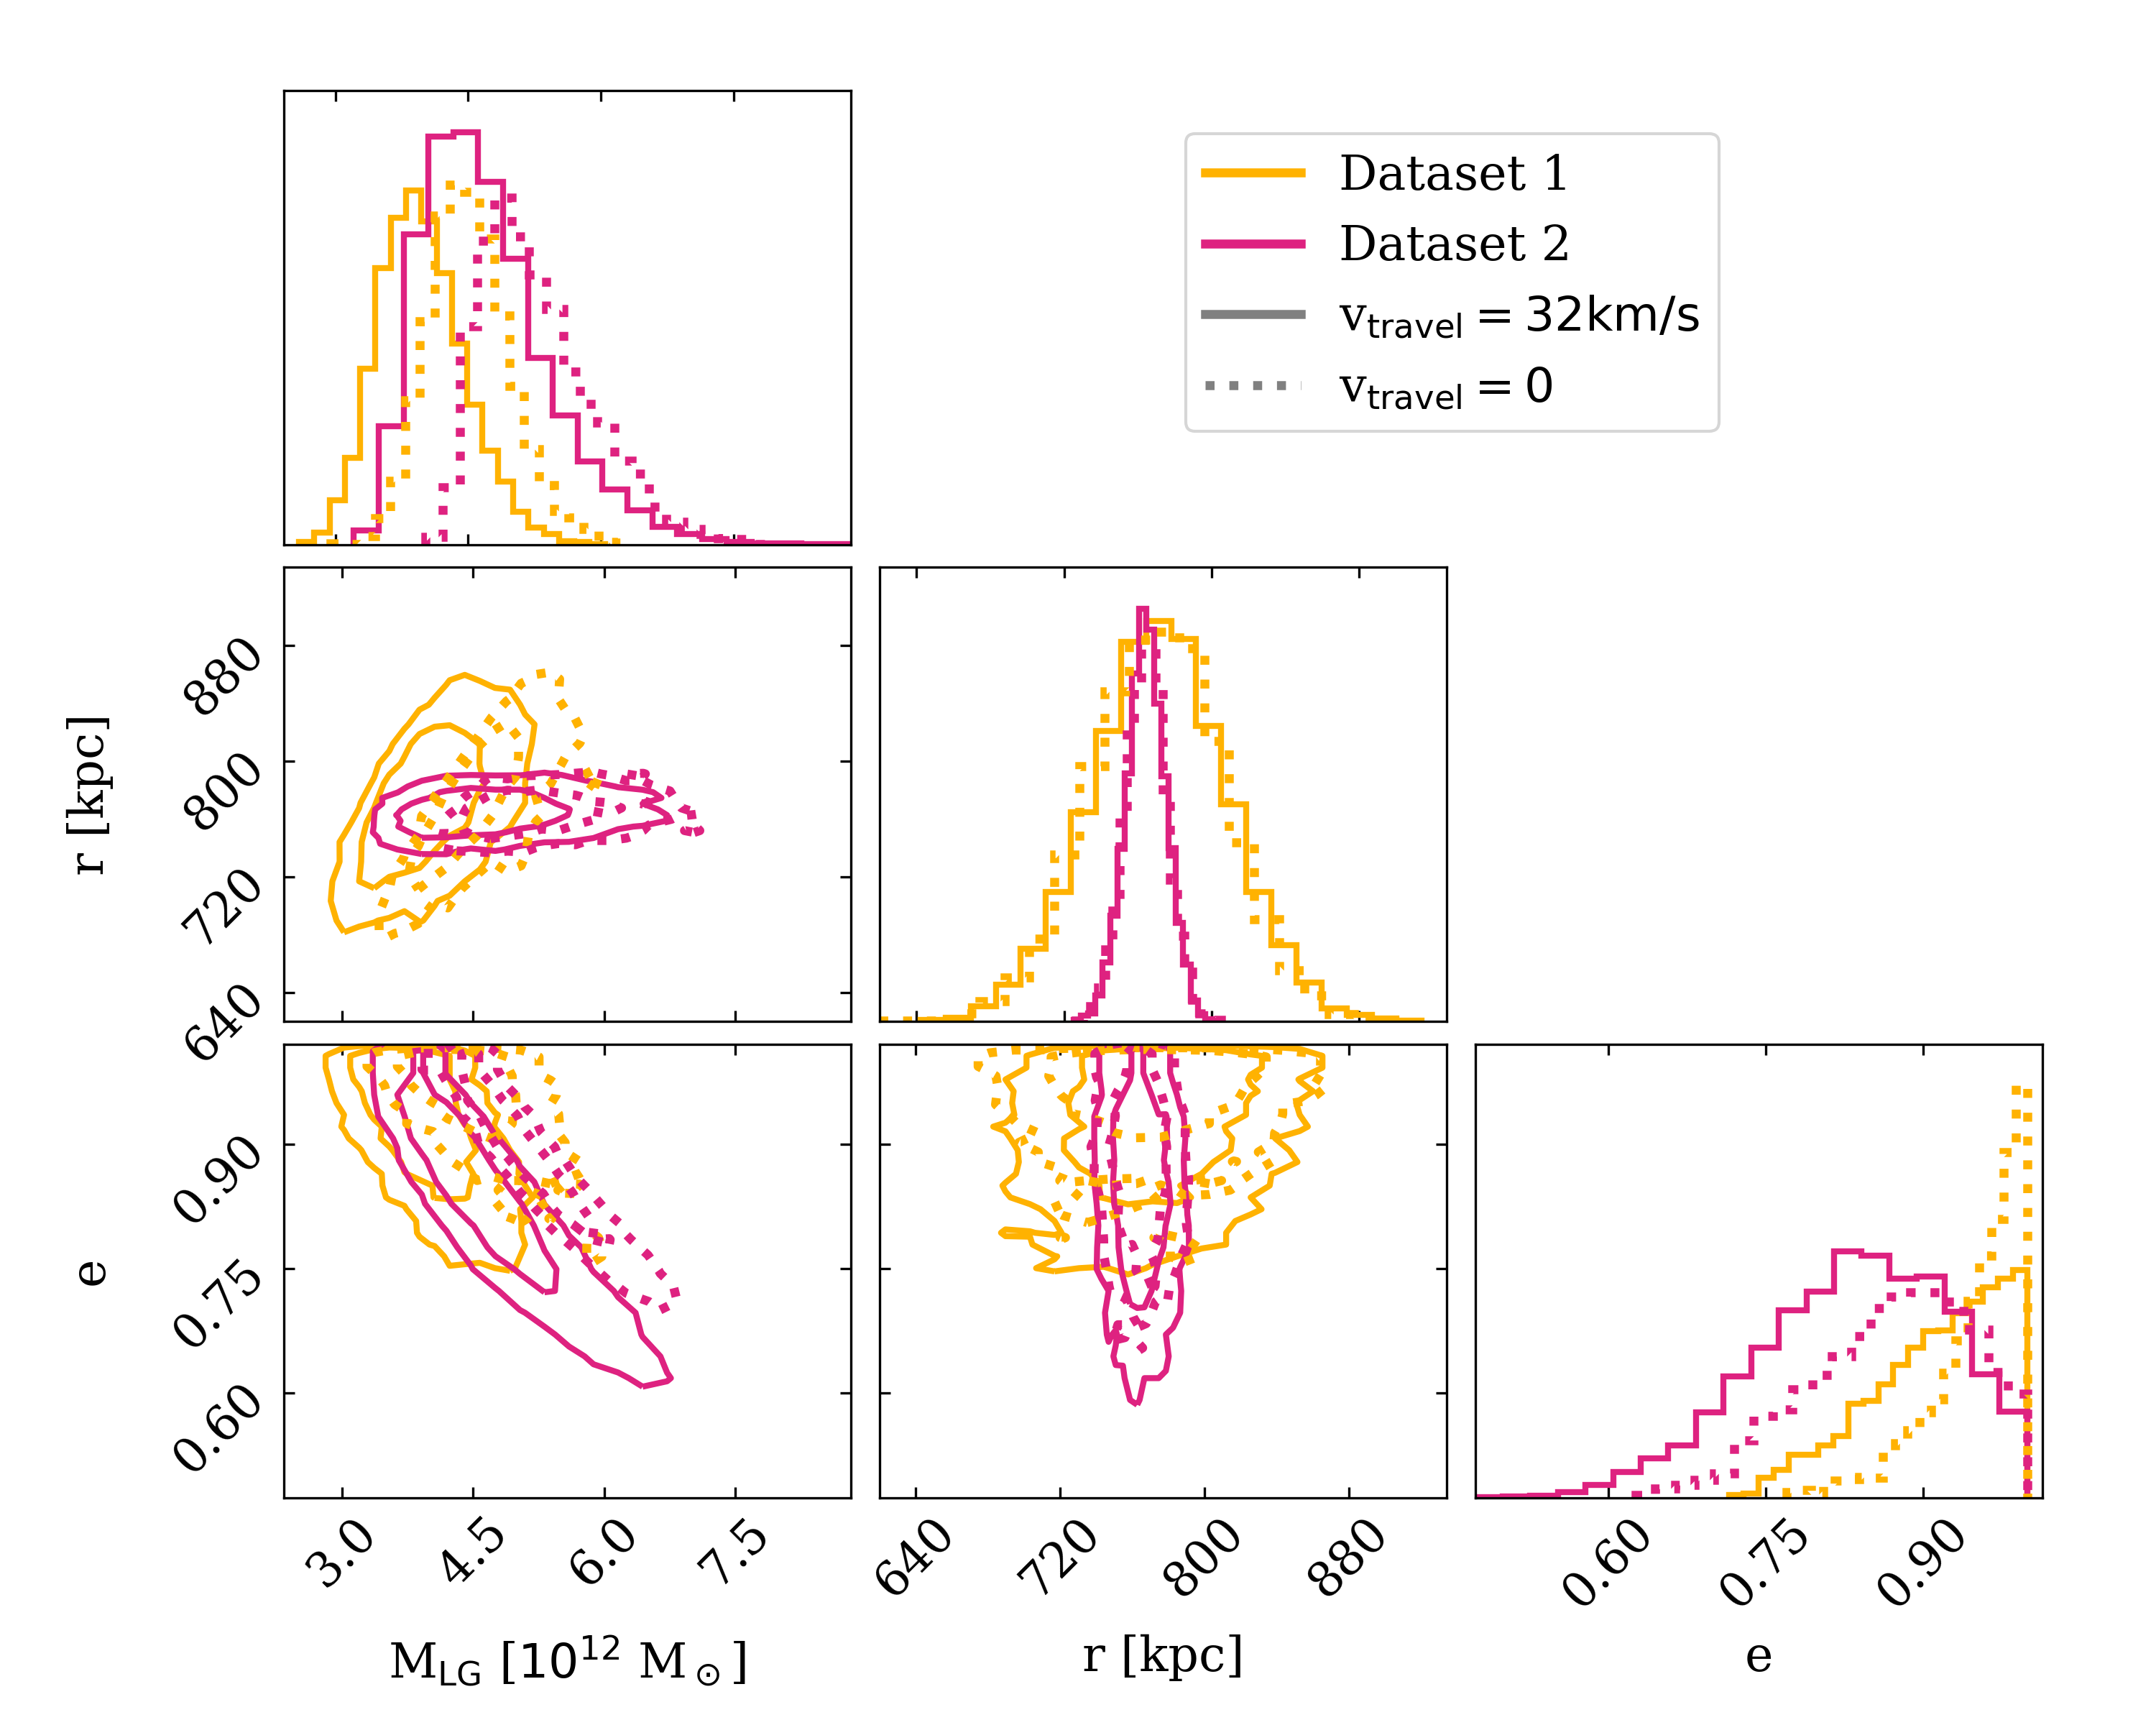
\includegraphics[width=\textwidth]{analyze-runs-contour.png}
  \caption{\label{fig:contour} Contours of sampled posterior distributions of the total mass of the Local Group (\mlg), the distance between the Sun and M31 ($r$), and the eccentricity of the orbit of M31 about a fixed MW ($e$), for two different observational datasets (yellow and pink).  \kc{need takeaway and more explanation}
  }
\end{figure*}

\begin{figure}[htb]
    \centering
    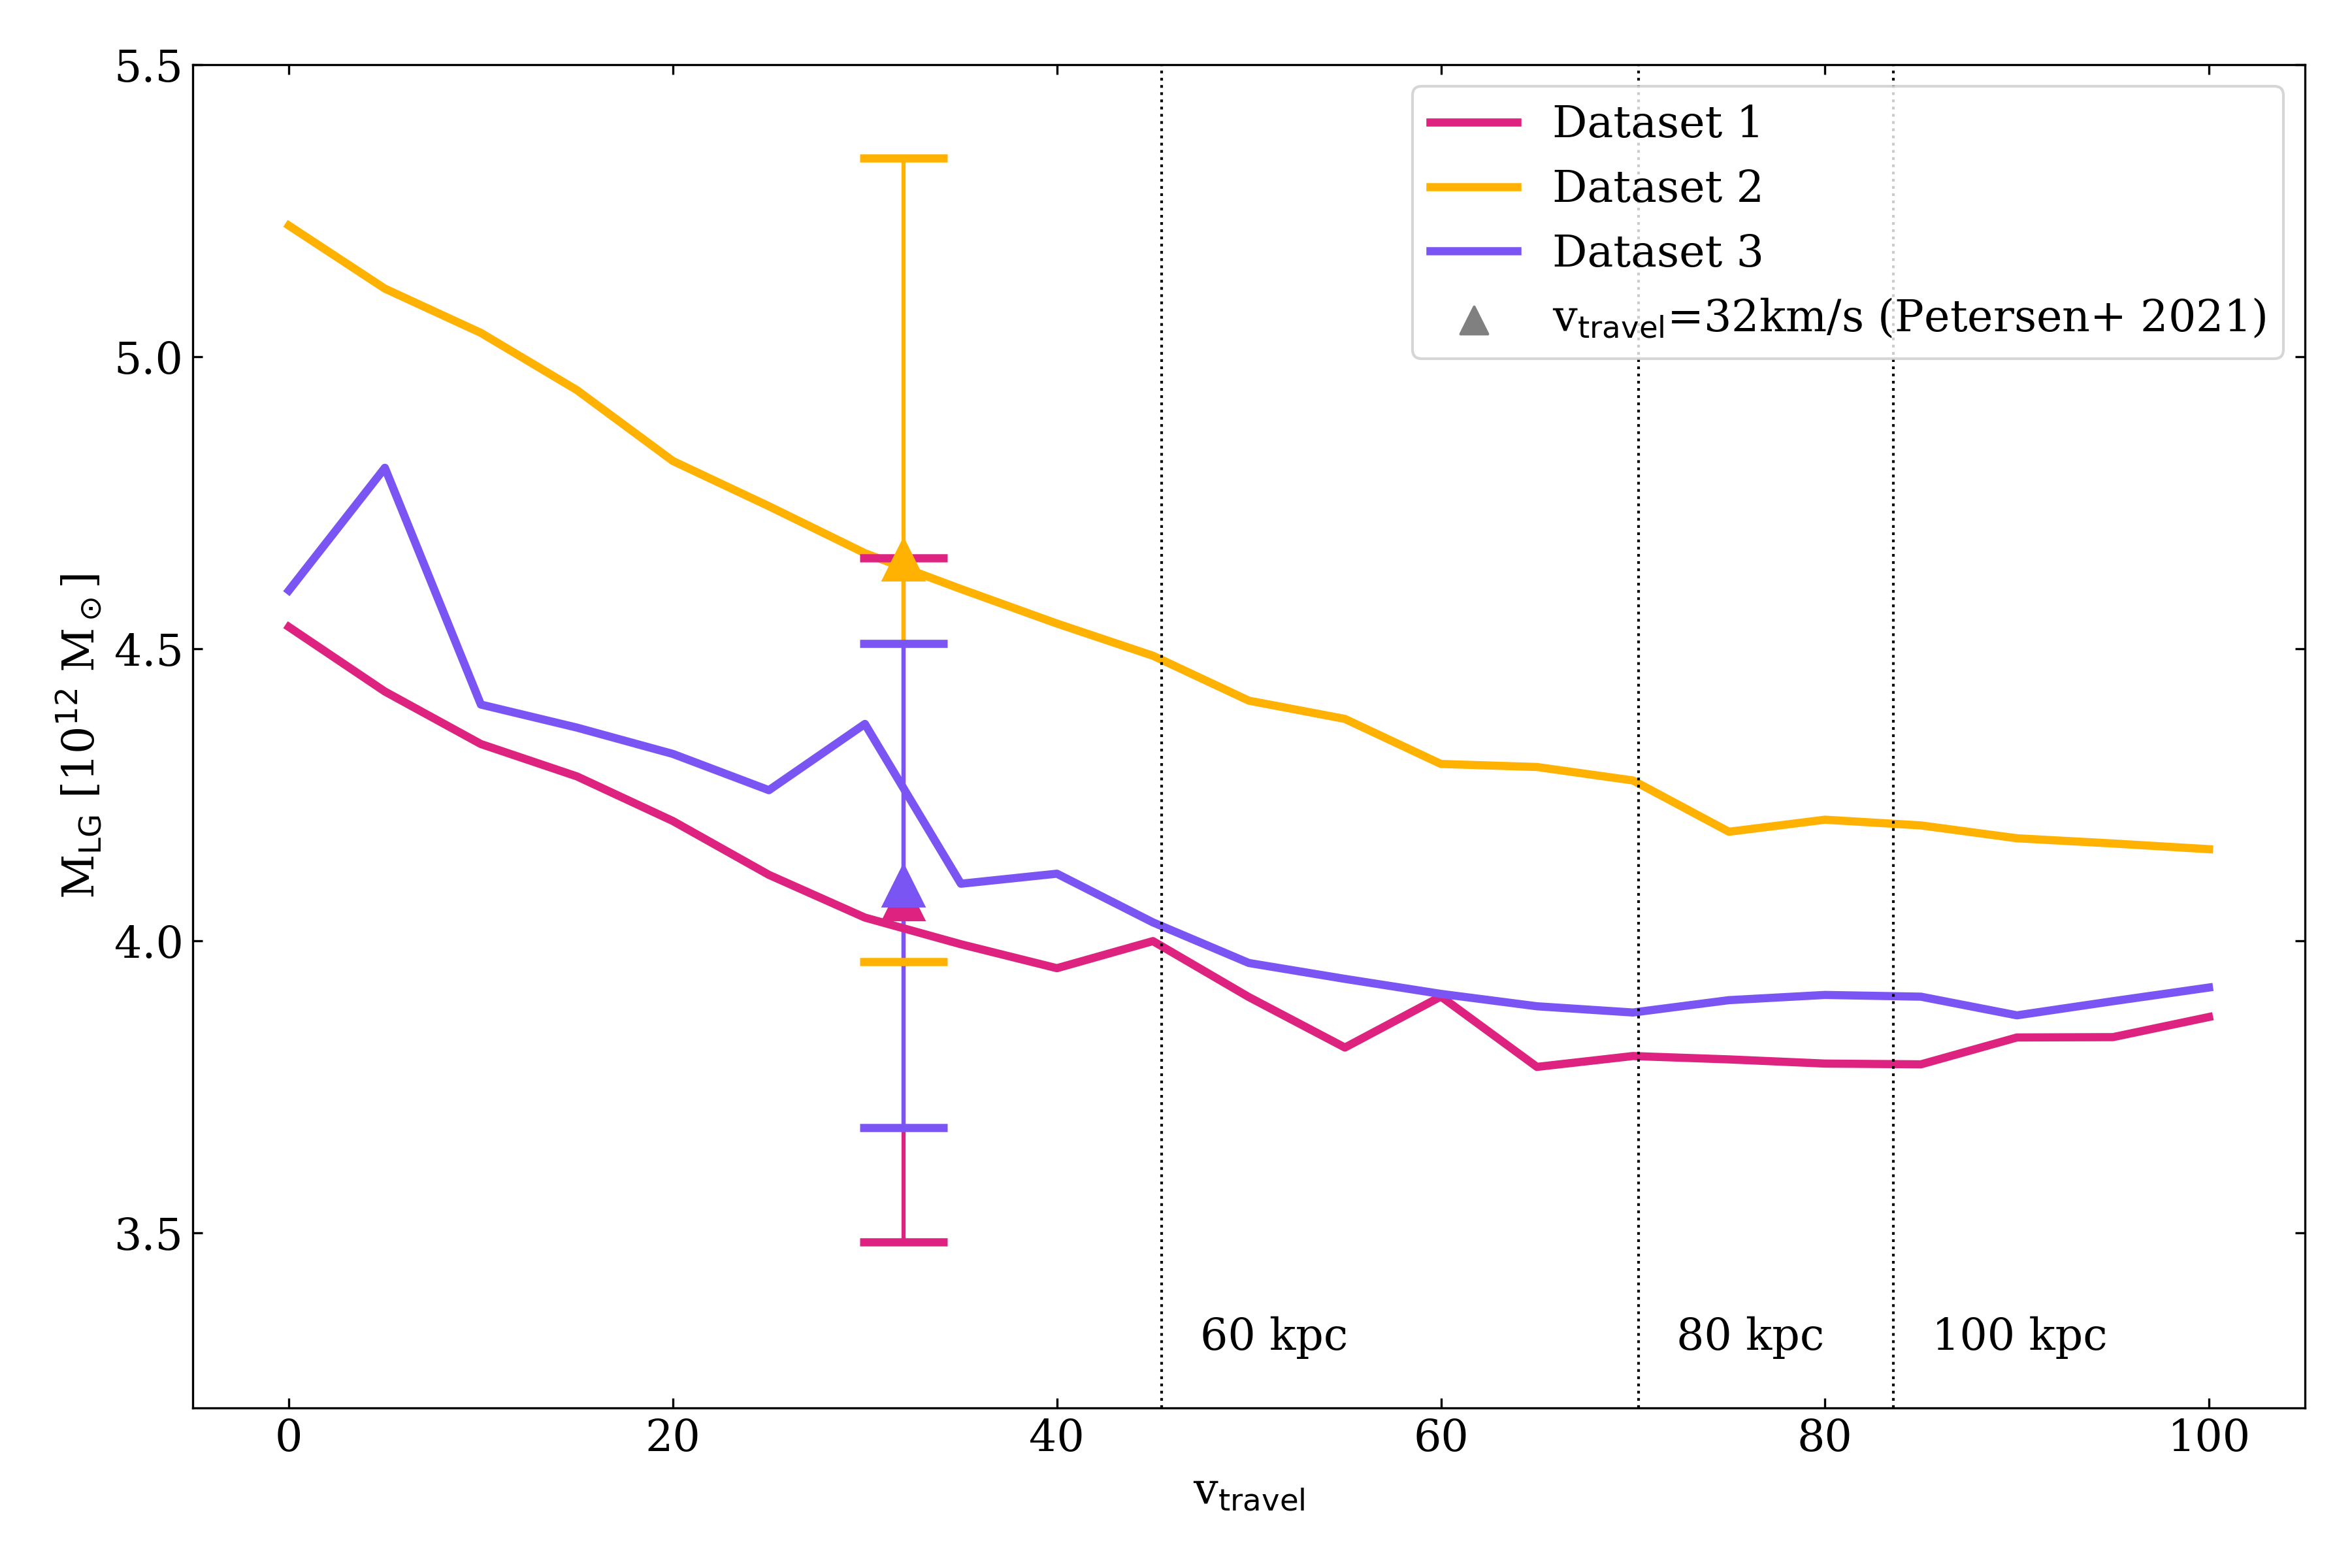
\includegraphics[width=\columnwidth]{analyze-runs-MvV.png}
    \caption{\label{fig:contour} \kc{add vertical lines with vtravel predictions from different tracer distances }
    }
  \end{figure}

\begin{figure}[htb]
    \centering
    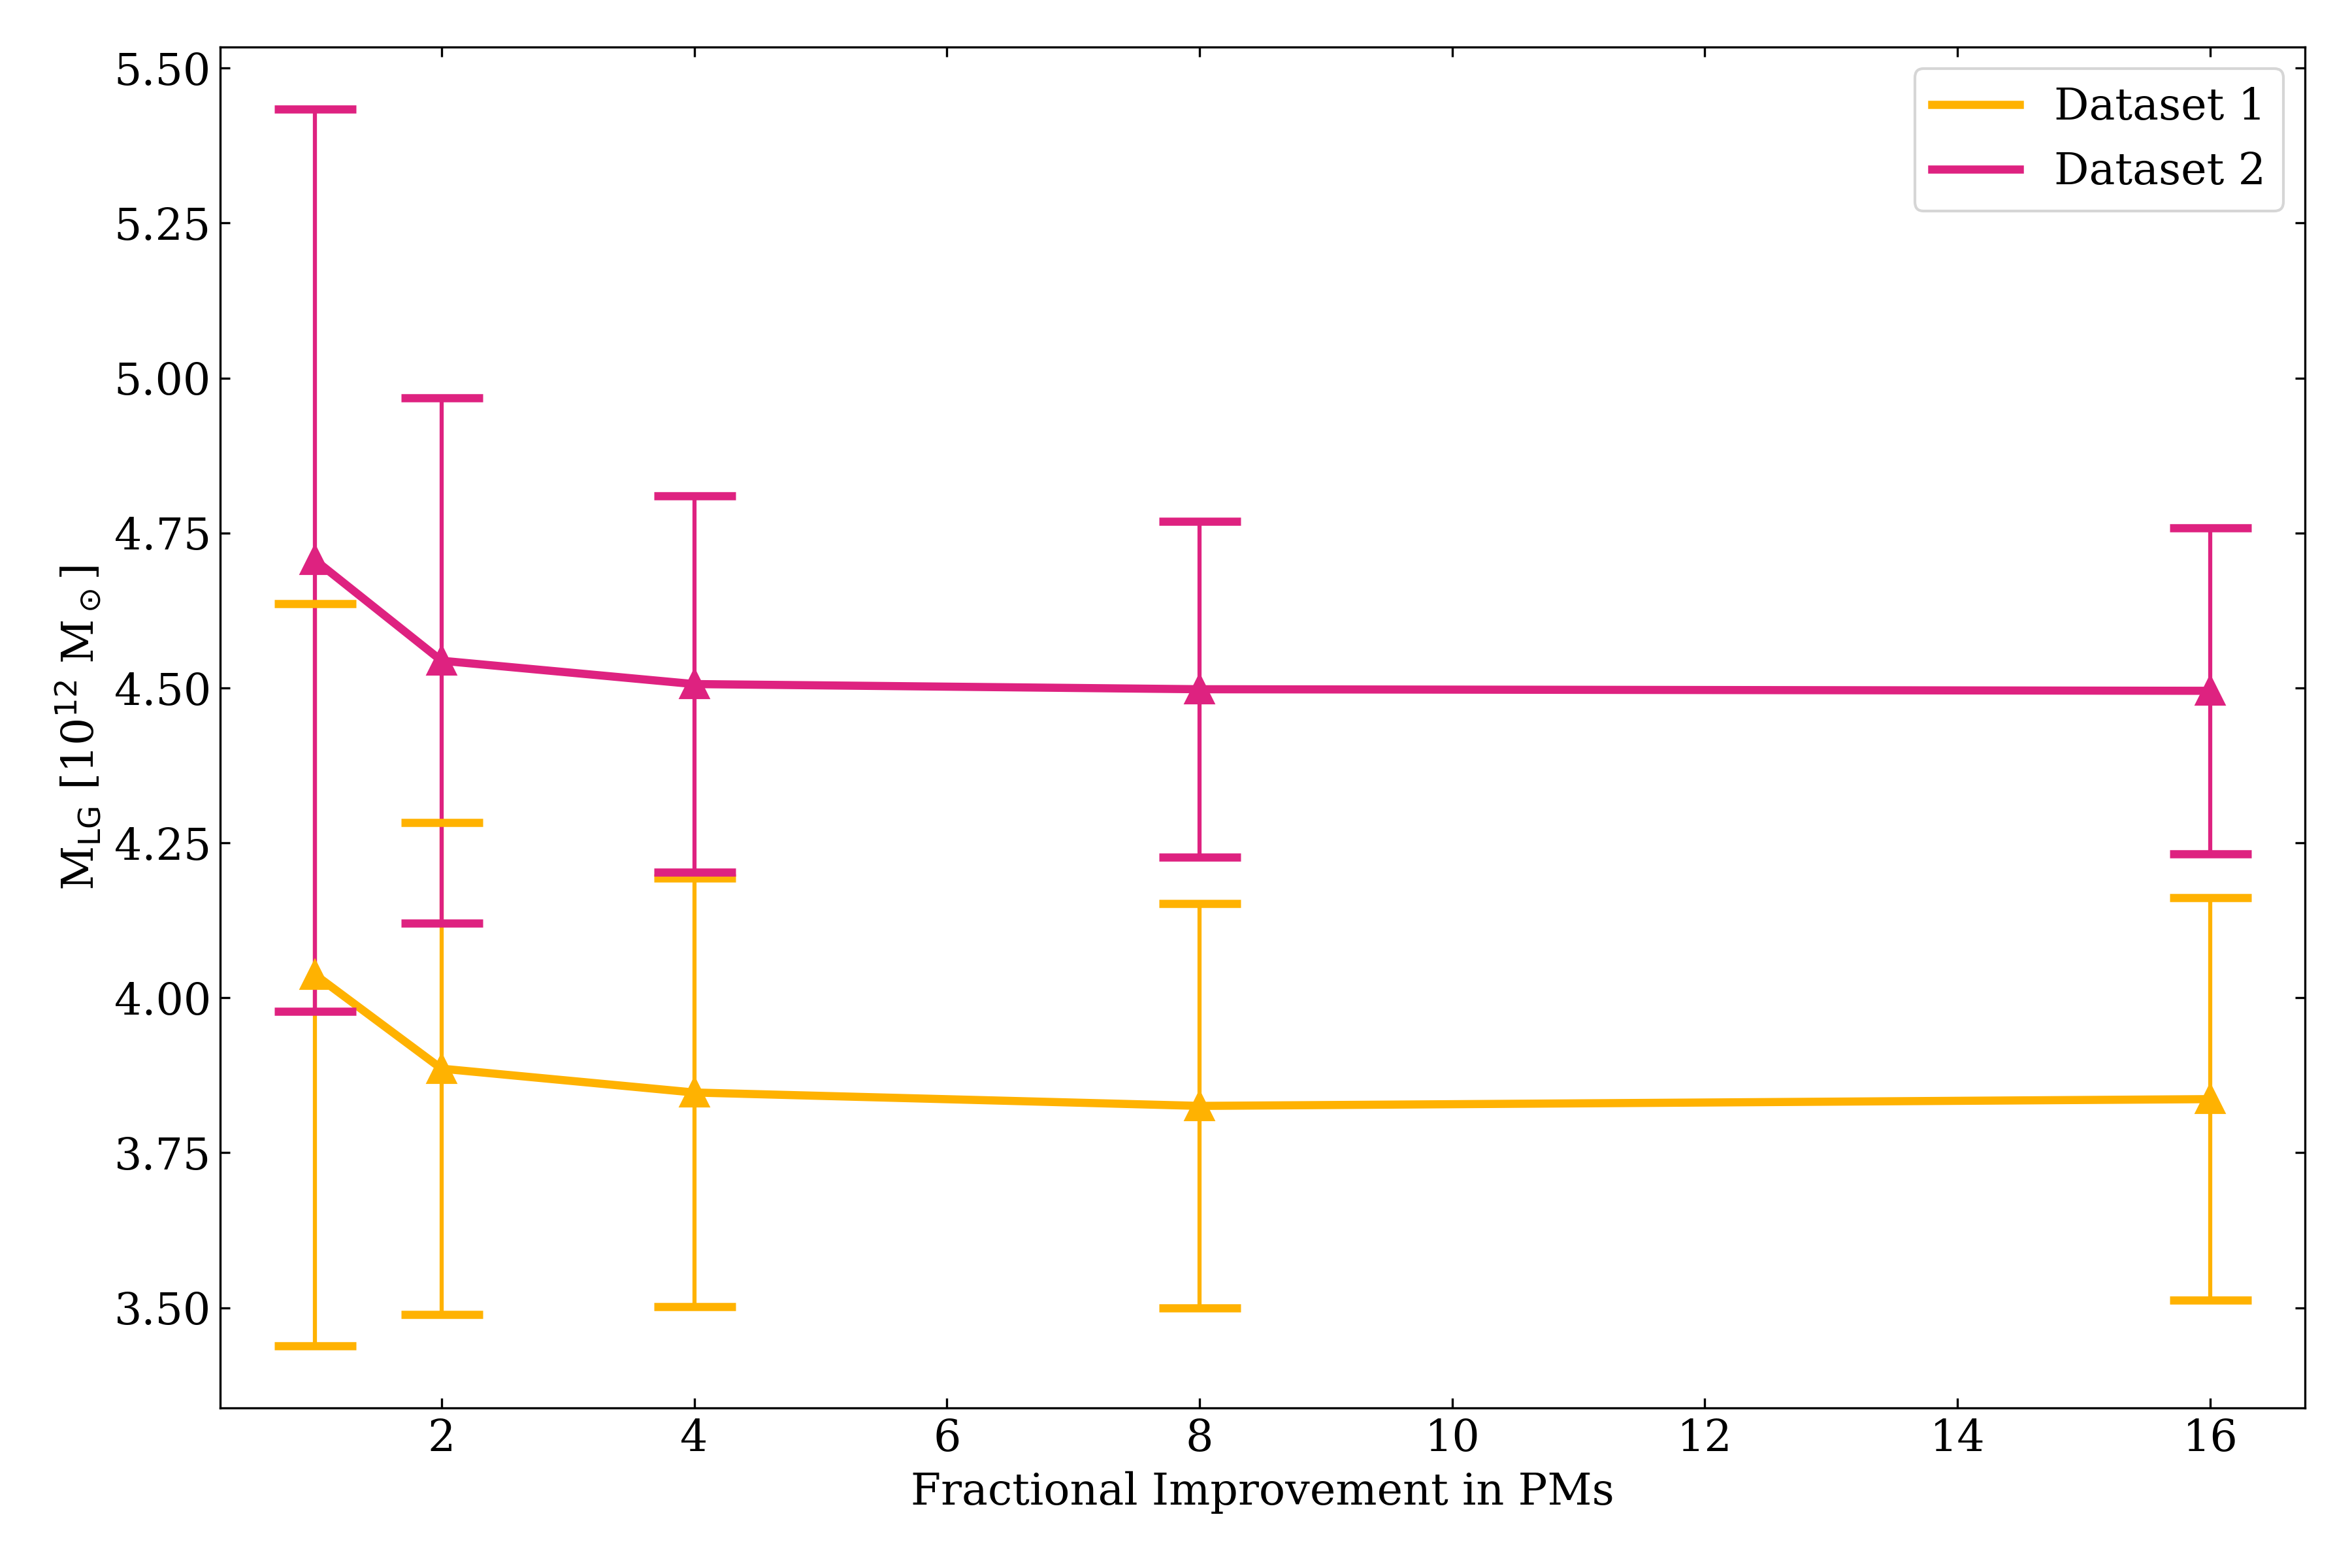
\includegraphics[width=\columnwidth]{analyze-runs-MvsPM.png}
    \caption{\label{fig:contour}
    }
\end{figure}


%%%%%%%%%%%%%%%%%%%%%%%%%%%%%%%%%%%
\section{Comparison to M33--M31 system}
%%%%%%%%%%%%%%%%%%%%%%%%%%%%%%%%%%%

%%%%%%%%%%%%%%%%%%%%%%%%%%%%%%%%%%%
\section{Summary and Discussion}
%%%%%%%%%%%%%%%%%%%%%%%%%%%%%%%%%%%
\label{sec:discussion}


% \software{
%     Astropy \citep{astropy, astropy:2018},
%     gala \citep{gala},
%     IPython \citep{ipython},
%     numpy \citep{numpy},
%     pymc3 \citep{Salvatier2016},
%     scipy \citep{scipy}
% }


\bibliography{refs}{}
\bibliographystyle{aasjournal}

\end{document}
